
\section{Interference Sources Select}\seclab{InterfSrc}

It is recommended to run the script \verb!"InterfSrcSel.sh"! using \verb!"InterfSrcSel.in"! as input to produce the plots that are zoomed in on the region of interest of the images made by the TRI-D imager, or to assemble the results of several TRI-D runs into a single image.

A typical input \verb!"InterfSrcSel.in"! resembles

\begin{linenumbers}
%\tiny
\resetlinenumber
\begin{verbatim}
&Parameters
 SMPowCut = 15e2 ! 5.e3
 AmpltPlot=10.
 MaxAmplFitPercent=0.001
 ZoomClip = .true.
 datafile=  "H99nw1",  "H99nw2"
 OutFileLabel="XYZ",
! xmin=-24.16 , xmax=-24.08, ymin=-10.25, ymax=-10.17, zmin=5.34, zmax=5.38  ! for NLa 37.10 37.6 -25.5 -25.25  5.35 5.8
!  tmin=606.552 , tmax=606.556
&End
xxxxxxxxxxxxxxxxxxxxxxxxxxxxx
\end{verbatim}
\end{linenumbers}

\begin{enumerate*}
\item[2] \verb!'SMPowCut = 15e2'!: Plot only those sources for which the intensity exceeds the specified limit.
\item[3] \verb#"AmpltPlot=10."#: The diameter of the largest symbols used in the plot. When zero or negative a fixed size dot will be used for all points, independent of their intensity.
\item[4] \verb!"! ZoomClip = .true."!: Only the points falling inside the plot boundary will be drawn.
\item[5] \verb#'datafile=  "H99nw1",  "H99nw2"'#: The \verb!"OutFileLabel="! from the different TRI-D runs for which the images have to be merged. This may also be just from a single run.
\item[6] \verb#'OutFileLabel="XYZ",'#: An additional label for the resulting plots, this in addition to the first entry in \verb#'datafile= '#.
\item[7] \verb#'! xmin=-24.16 , xmax=-24.08,'#: The boundaries of the plots will be taken from the first entry in \verb#'datafile= '# but will be overwritten if any of these settings is activated.
\end{enumerate*}

\subsection{Figures and print-out}%\seclab{RFI-out}

The produced .dat files are plain text files and contain some header lines with some general information followed by the specific data of the sources. The files have a format that is suitable for the plotting script \verb!"SourcesPlot.gle"!. 

The out file \verb#'IntfrSrcSel.out'# looks like

\begin{linenumbers}
\tiny
\resetlinenumber
\begin{verbatim}
 ======================  Mx_d
 After file:files/IntfSpecPowMx_d.dat, SourcTotNr=          59
 Time span data=   343.94184999999999        343.94967000000003
Amplitudes (#=      59), max@ 198243.0, 5-pctile@********, 10-pctile@87401.70
Amplitude with   0.001pctile as included in fit @********
 $b *exp(-a*A-c/A^2); \chi^2=$  0.98,with  a,b,c=  0.0023 0.903E-05   0.00    ; nrm=  0.805E+05
 $b *A^-a *exp(-c/A); \chi^2=$  0.97,with  a,b,c=   4.023 0.156E+07   0.00    ; nrm=  0.805E+05
 $b *exp(-a*A-c/A^2); \chi^2=$  0.98,with  a,b,c= 0.2304E-020.9031E-05   0.00    ; nrm=   6.10      0.805E+05
 $b *A^-a *exp(-c/A); \chi^2=$  0.97,with  a,b,c=  4.023    0.1562E+07   0.00    ; nrm=   7.04      0.805E+05
 number of sources in plots:          59   1000.0000000000000      Mx_dIntfSpecSel
 ======================  End input
\end{verbatim}
\end{linenumbers}

Showing the number of points that fall within the plot boundary. A fit is made to the power spectrum for different functional dependencies and the resulting parameters are specified.

Two gle-scripts \verb#'%UtilDir%Intensity.gle'# and \verb#'%UtilDir%SourcesPlot.gle'# make the following plots.

\begin{figure}[h]
\setlength{\unitlength}{.48\textwidth} % .43\textwidth}
   \subfloat[Figure `IntfSpecSel']{ 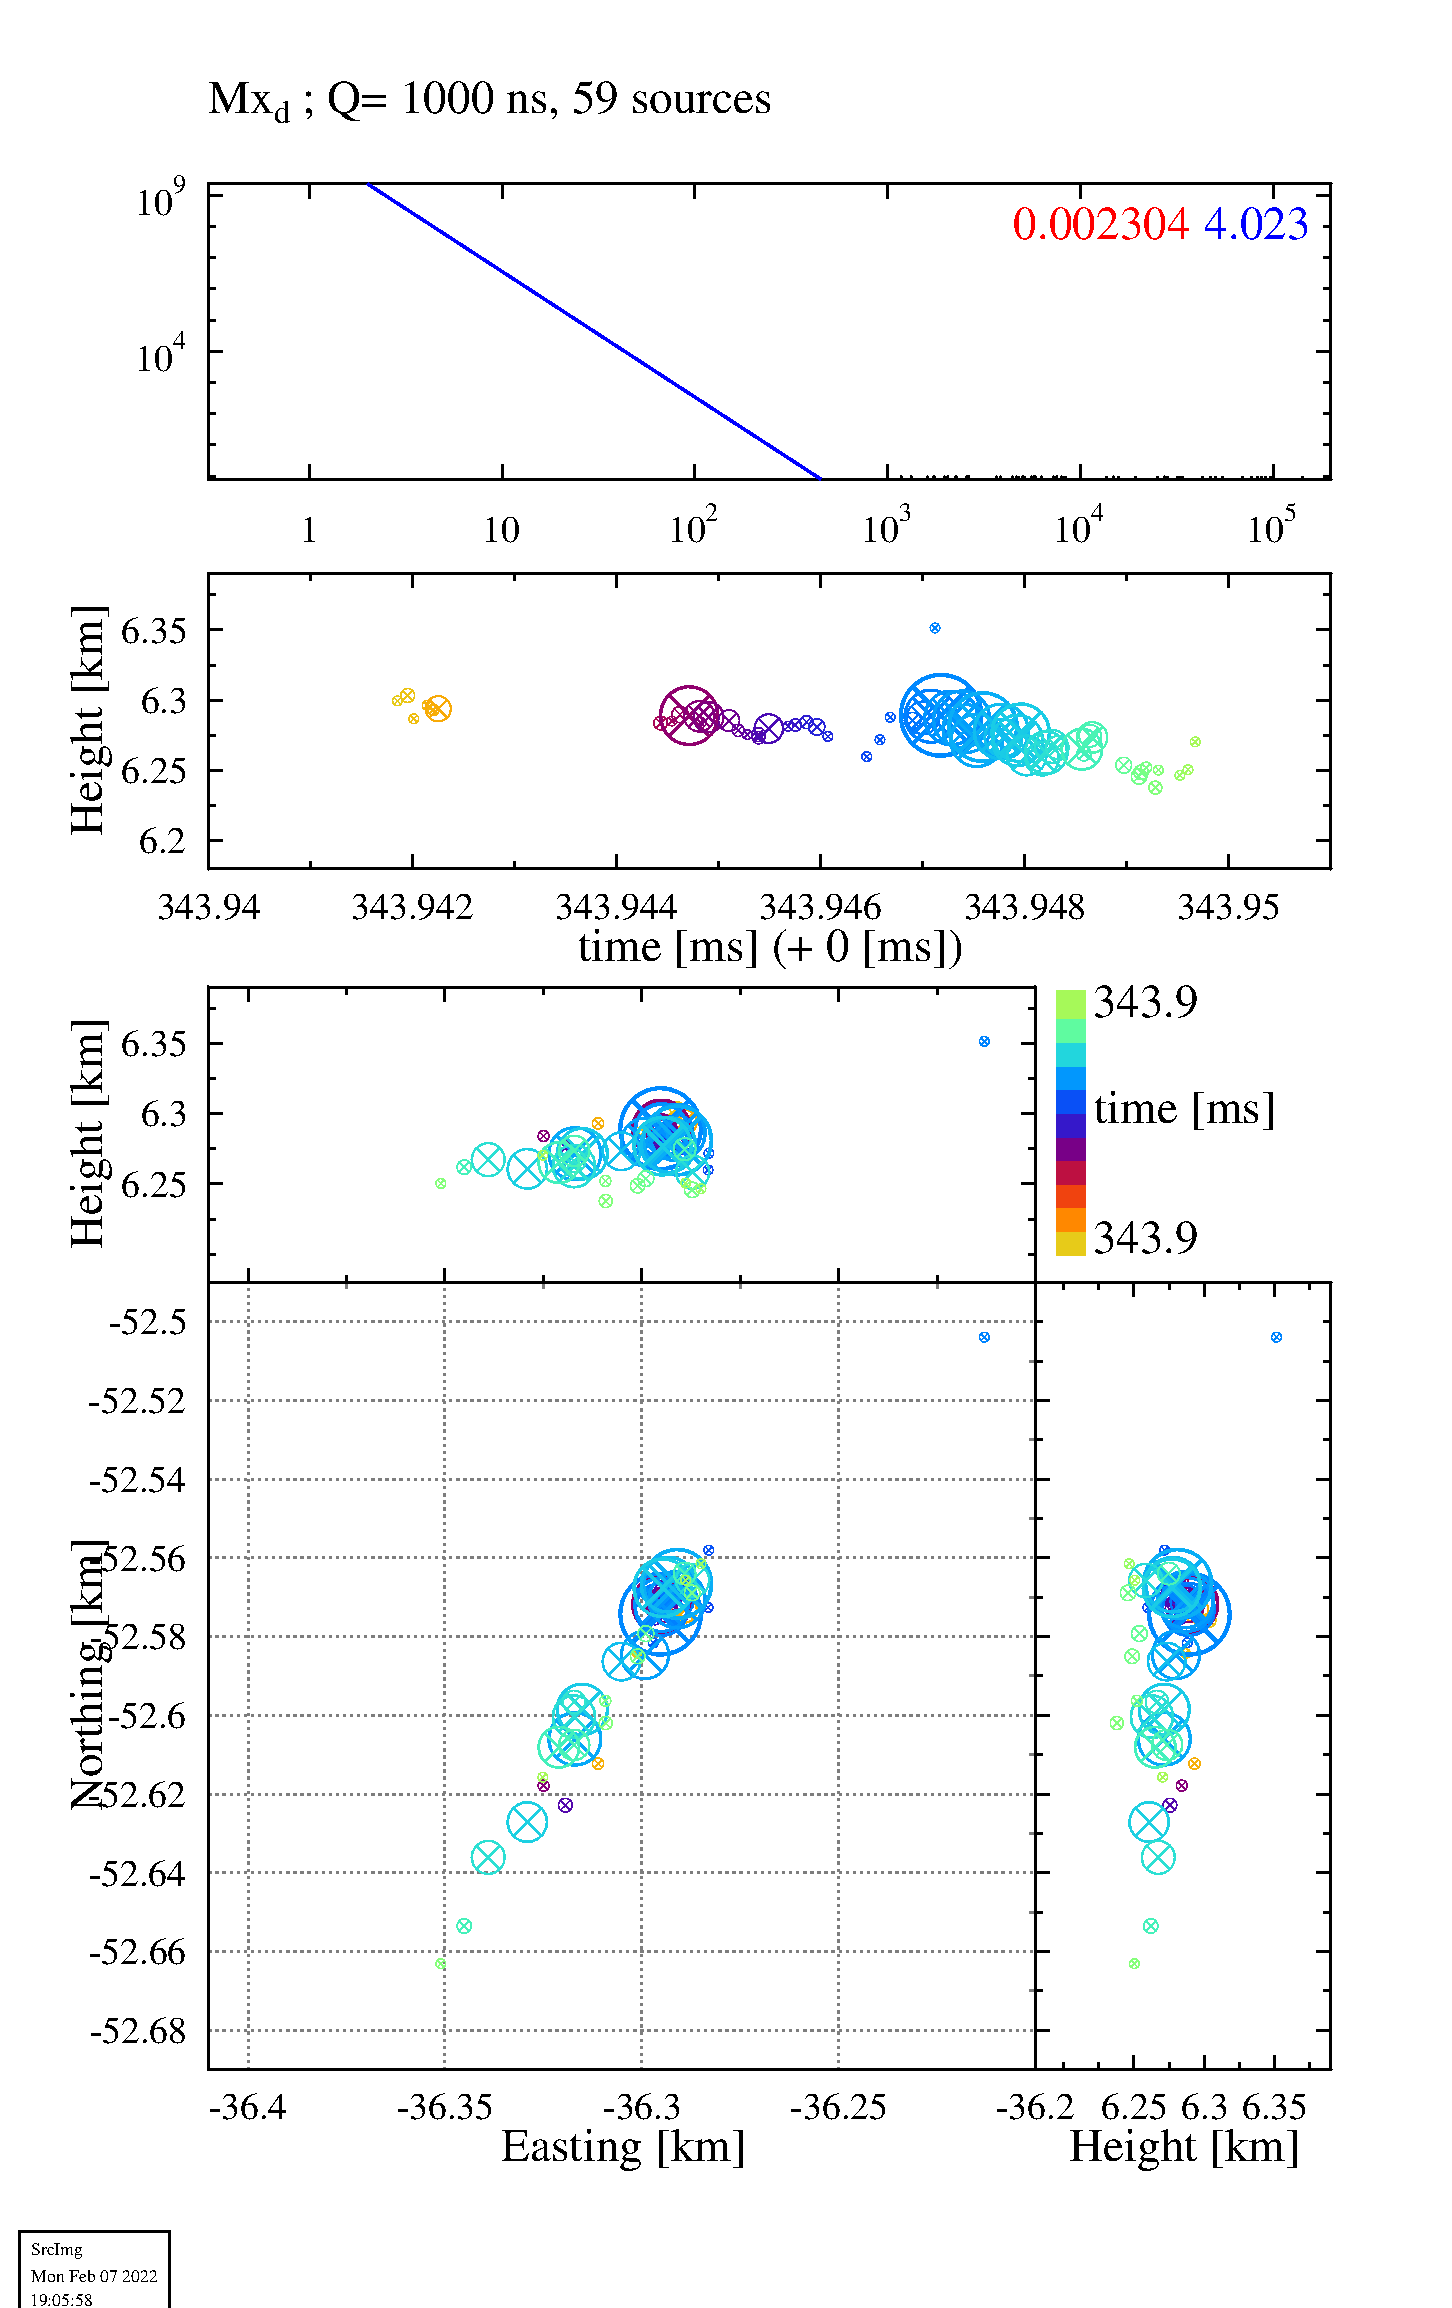
\includegraphics[width=\unitlength]{Figs/Mx_dIntfSpecSel}  \figlab{InterfSrc-Spec}}
   \subfloat[Figure `AmplFit']{ 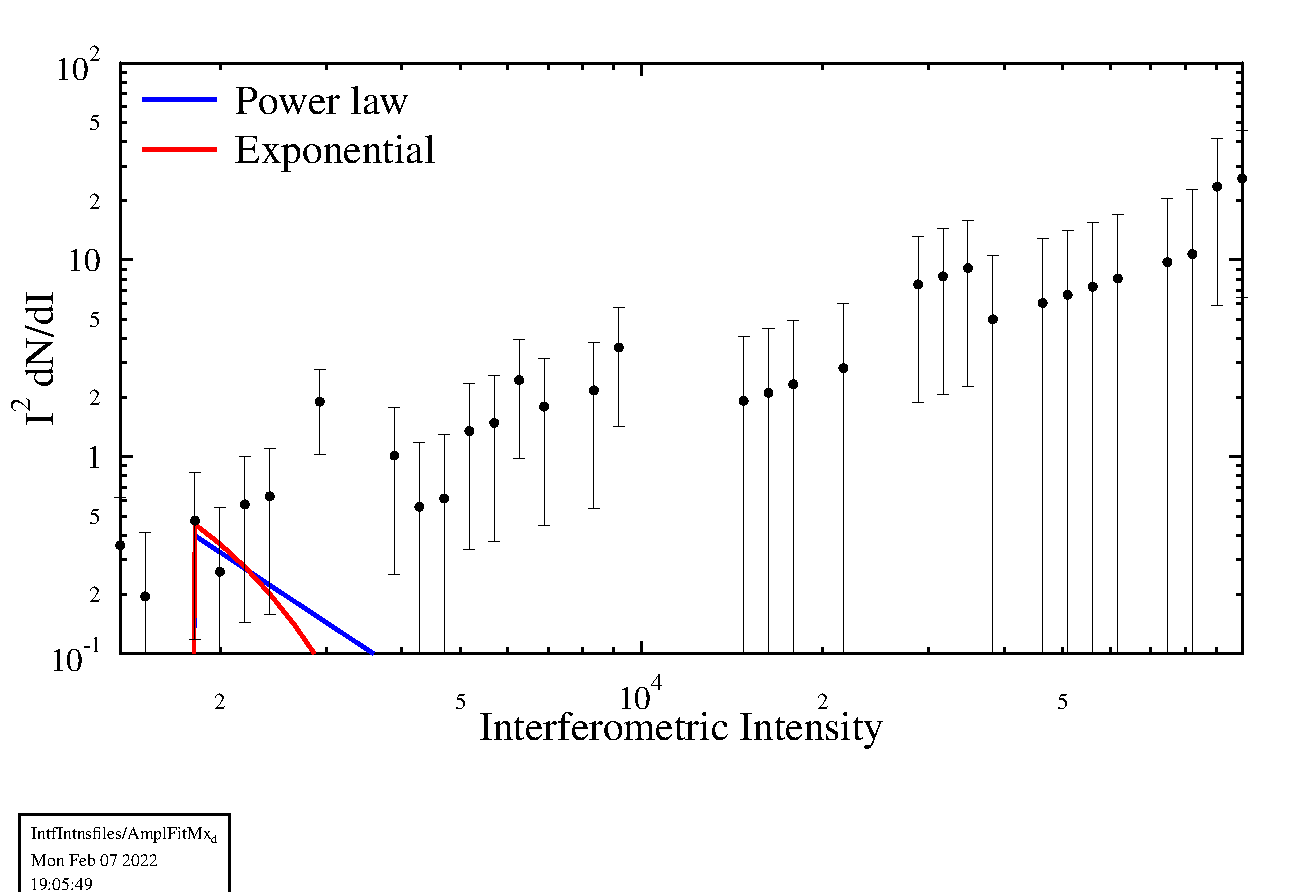
\includegraphics[width=\unitlength]{Figs/Mx_dAmplFit}  \figlab{InterfSrc-Ampl}}
	\caption{Top panel in \figref{InterfSrc-Spec} shows the intensity distribution of the sources and two fits (that obviously do not resemble the data for this case). The lower panels the usual way of plotting the sources where the size of the circles reflects the intensity.
\figref{InterfSrc-Ampl} displays an attempt to fit the pulse-strength distribution.}	 \figlab{InterfSrc}
\end{figure}

\clearpage
